%!TEX root = ../sbc-template.tex

A contextualização bibliográfica para a realização deste trabalho compreende conceitos ligados ao \emph{
Deep Learning}. Assim, a Seção \ref{sec:dl} introduz os conceitos essenciais relativos à área. Os conceitos relativos específicamente às redes neurais convolucionais são descritos na Seção \ref{subsubsec:rnc}. Alguns trabalhos relacionados à estimação de idade por meio de fotografias faciais estão descritos na Seção \ref{sec:trab_relac}.

% \section{\emph{Machine Learning}} \label{sec:machineLearning}
% %!TEX root = ../sbc-template.tex

\emph{Machine Learning} (ML), também chamado de Aprendizado de Máquina, é uma subárea da Inteligência Artificial que trata do estudo sistemático de algoritmos e sistemas que são capazes de melhorar seu desempenho com a experiência. Um algoritmo neste domínio é capaz de aprender a partir de dados, capturando padrões e efetuando inferências. Estes algoritmos podem ser entendidos em uma analogia com  humanos e outros animais que, ao se depararem com determinada situação, costumam procurar lembranças de situações similares, de como agiram, e se o comportamento adotado foi vantajoso, e deve ser repetido, ou prejudicial, devendo ser evitado \cite{marsland2015machine,goodfellow2016deep,flach2012machine}.

Para consolidar o aprendizado, os algoritmos de \emph{machine learning} precisam passar por um processo de aquisição da experiência, comumente chamado de treinamento. De acordo Mitchell \cite{mitchell1997machine}, um algoritmo que aprende a partir da experiência $E$ quanto a um conjunto de tarefas $T$ e medida de performance $P$, se sua performance nas tarefas em $T$, medida por $P$, melhora com a experiência $E$.

Ao preparar um algoritmo de \emph{machine learning} para desenvolver determinada tarefa, busca-se um modelo, ou seja, uma função, que mapeie as instâncias do espaço de entrada para o de saída \cite{flach2012machine}. Estes modelos podem ser agrupados em diferentes categorias ao se considerar o tipo de aprendizado e também a saída desejada para o algoritmo. A Figura \ref{fig:ml_algorithms} apresenta uma visão geral do estado da arte acerca dos modelos de ML e suas subdivisões.

\begin{sidewaysfigure}
	\includegraphics[width=\linewidth]{img/machinelearningalgorithms.png}
	\caption{Mapa mental dos algoritmos de \emph{Machine Learning} organizados por área e sub-área.}
	\label{fig:ml_algorithms}
\end{sidewaysfigure}

Quanto ao tipo de aprendizado, as tarefas de ML podem ser agrupadas em três tipos diferentes, a depender da presença e do tipo de resposta dada ao algoritmo quanto ao desempenho de suas saídas. No \emph{aprendizado supervisionado}, o algoritmo deve aprender a inferir valores a partir de atributos preditores e do respectivo atributo alvo fornecido como exemplo, ou seja, de cenários em que se têm seus valores de saída conhecidos. Os modelos mais comumente utilizados neste tipo de aprendizado são as máquinas de vetores de suporte, redes neurais artificiais \emph{feed-forward}, regressão linear e logística, etc. Já no \emph{aprendizado não-supervisionado}, o algoritmo deve inferir padrões e estruturas a partir de dados não rotulados, buscando alguma estrutura interna que caracterize os dados. Exemplos de modelos aplicáveis a este cenário são os algoritmos \emph{k-means} e \emph{k-medoids}.  Por fim, no \emph{aprendizado por reforço} o algoritmo não recebe dados nem tampouco rótulos, e deve aprender a partir das recompensas positivas ou negativas dadas por ações que modifiquem o ambiente de maneira satisfatória ou não \cite{flach2012machine}.

Quanto ao tipo de saída desejada, os problemas que podem ser endereçados segundo ML são de classificação, regressão, transcrição, tradução automática, detecção de anomalia, síntese e amostragem. No caso do aprendizado supervisionado, em particular, as principais tarefas realizadas são de classificação e regressão \cite{flach2012machine}.

Um algoritmo proposto a uma tarefa de classificação deve especificar cada entrada $x$ como pertencente a uma dentre $k$ categoritas pré-determinadas, produzindo uma saída $y=f(x)$ tal que a função $f$ é definida como $f: \mathds{R}^n \rightarrow \{1, \ldots, k\}$, ou seja, $f$ mapeia sequências de números reais  $x$ de dimensão $n$ para um valor inteiro $y$ dentre $k$ possibilidades \cite{goodfellow2016deep}. Dentre as tarefas de classificação estão, por exemplo, o reconhecimento de objetos em uma imagem, determinar se um indivíduo será ou não vítima de determinada doença, se sobreviverá ou não a determinado acidente, etc.

Numa tarefa de regressão, por sua vez, objetiva-se aprender uma função de valor real a partir de uma entrada \cite{flach2012machine}. Assim, a saída $y=f(x)$ é dada pela função $f: \mathds{R}^n \rightarrow \mathds{R}$, ou seja, $f$ mapeia uma entrada multidimensional $x$ para um valor $y$ real \cite{goodfellow2016deep}. Algumas tarefas de regressão envolvem a previsão de preços de um mercado de ações, a determinação do risco do seguro para um carro, do volume diário de precipitação em determinada cidade, etc.

Os modelos de ML são organizados em dois grandes grupos, dos tipos paramétricos ou não paramétricos. Segundo Russel e Norvig, um modelo de aprendizado que resume dados utilizando um conjunto de parâmetros de tamanho definidos independente do número de exemplos de treinamento é chamado de \emph{modelo paramétrico}. Dentre os modelos paramétricos está a regressão logística. Já um \emph{modelo não-paramétrico}, por sua vez, é aquele que não pode ser caracterizado por um conjunto limitado de parâmetros. Alguns exemplos de modelos não-paramétricos são máquinas de vetores de suporte, redes neurais artificiais, $k$ vizinhos mais próximos e árvores de decisão CART e C4.5 \cite{russell2016artificial}.

Dentre os modelos não paramétricos, as redes neurais artificiais têm demonstrado resultados satisfatórios em tarefas de classificação e regressão quando aplicadas em diversas áreas. Em especial, aplicações de \emph{Deep Learning} no reconhecimento de objetos e no processamento de linguagem natural, por exemplo, têm trazido ainda mais atenção a este modelo. Diante desta importância e da utilização no contexto deste trabalho, estes conceitos serão abordados com mais profundidade nas seções a seguir.

%
% \subsection{Redes Neurais Artificiais} \label{sec:rnas}
% %!TEX root = ../sbc-template.tex

%conceito, inspiração biológica
Redes Neurais Artificiais (RNAs) são um modelo de computação não algorítmica caracterizado por sistemas que, em algum nível, lembram a estrutura do cérebro humano. São sistemas pararelos distribuídos compostos por unidades de processamento simples, os neurônios, que calculam funções matemáticas, normalmente não-lineares. Estes neurônios são dispostos em uma ou mais camadas e interligados por um grande número de conexões normalmente unidirecionais e comumente associadas a pesos que armazenam o conhecimento representado no modelo e ponderam a entrada recebida por cada neurônio da rede. Os principais atrativos das RNAs envolvem a capacidade de capturar tendências a partir de um conjunto de exemplos e dar respostas coerentes para dados não-conhecidos, ou seja, de generalizar a informação aprendida.

A motivação para a criação deste modelo vem do funcionamento do cérebro biológico, que é formado por neurônios interligados que se comunicam entre si de modo contínuo e paralelo através de impulsos nervosos. Esta complexa rede neural biológica é capaz de reconhecer padrões e relacioná-los, produzir emoções, pensamentos, percepcção e cognição, além do . Cada neurônio é composto de um corpo, dendritos e um axônio, como é mostrado na Figura \ref{fig:neuronio_biologico}. Os dendritos são responspaveis pela recepção de impulsos nervosos vindos de outros neurônios; o corpo combina os sinais recebidos pelos dendritos e caso o resultado ultrapasse determinado limiar de excitação do neurônio, são gerados novos impulsos nervosos, que são transmitidos pelo axônio até os dendritos dos neurônios seguintes. Esta conexão unilateral entre neurônios biológicos está expressa na Figura \ref{fig:redeneuralbiologica}.

\begin{figure}[ht]
	\centering
	\includegraphics[height=0.3\textheight]{img/neuronio}
	\caption{Neurônio biológico e seus componentes: corpo, axônio e dendritos.}
	\label{fig:neuronio_biologico}
\end{figure}

\begin{figure}[ht]
	\centering
	\includegraphics[width=0.6\textwidth]{img/redeneuralbiologica.jpg}
	\caption{Conexão entre neurônios biológicos}
	\label{fig:redeneuralbiologica}
\end{figure}

\begin{figure}[ht]
	\centering
	\includegraphics[width=0.7\textwidth]{img/perceptron.png}
	\caption{Representação de um neurônio}
	\label{fig:neuronio}
\end{figure}

Com base neste modelo biológico, McCulloch e Pitts propuseram em \cite{mcculloch1943logical} um neurônio artificial. Explanado na Figura \ref{fig:neuronio}, o modelo de McCulloch e Pitts é formado por somente um neurônio artificial que contém $n$ terminais de entrada dada por $ x = x_1, \ldots, x_n$ e um terminal de saída $y$. Esta organização faz uma alusão aos dendritos, centro e axônio de um neurônio biológico. A saída é mapeada através de uma função de ativação $y = g(z)$ expressa na Equação \ref{eq:funcao_neuronio}, em que a soma ponderada $z$ do vetor de entrada $x$ pelo conjunto de pesos $w = w_1, \ldots, w_n$ deve ser maior ou igual a um limiar de ativação $\theta$.

\begin{gather}\label{eq:funcao_neuronio}
	z = \sum_{i=1}^n x_i w_i\\
	y = g(z) =
		\begin{cases}
			0, & \text{se } z < \theta\\
			1, & \text{se } z \geq \theta
		\end{cases}
\end{gather}

Em 1958, Frank Rosenblatt apresenta o neurônio \emph{Perceptron} \cite{rosenblatt1958perceptron}, que mais tarde seria empregado como a unidade de processamento de uma RNA e de outros modelos de ML como as \emph{support vector machines}. O Perceptron agregou ao neurônio de McCulloch e Pitts conceitos cruciais para a caracterização das RNAs como são conhecidas hoje, como a não obrigatoriedade de igualdade dos pesos e limiares de ativação, a possibilidade de os pesos serem positivos ou negativos, a diversidade de funções de ativação, entre outros. Sua maior contribuição envolve a adição de um algoritmo de aprendizado, que permite a adaptação de seus pesos para que a rede possa se aproximar de uma função que exiba saídas adequadas para determinada tarefa de aprendizado dadas as entradas do conjunto de dados \cite{braga2000redes}.

\begin{enumerate}
	\item Inicializar a taxa de aprendizado $\eta$ e o vetor de pesos $w$;
	\item Para cada par do conjunto de treinamento $(x, y)$:
	\begin{enumerate}
		\item Atualizar o vetor de pesos para cada um dos neurônios da rede segundo a regra
		\begin{equation}\label{eq:regra_aprendizado}
			w(t+1) = w(t) + \eta e x(t)
		\end{equation}
		até $e = 0$ para todos os $p$ elementos do conjunto de treinamento em todos os neurônios da rede.
	\end{enumerate}
\end{enumerate}

\todo[inline]{Linkar com backpropagation --> gradiente descendente, solvers}
\todo[inline]{introduzir a noção de camadas de neurônios}

Este modelo inicial apresentava algumas limitações, atribuídas principalmente à sua linearidade e simplicidade, características que possibilitam resolver apenas problemas linearmente separáveis \cite{braga2000redes}. Um modelo Perceptron é incapaz de aprender a função XOR, por exemplo \cite{goodfellow2016deep}. Atualmente, as redes neurais artificiais podem apresentar diversos tipos de arquitetura, ao variar parâmetros como o número de camadas de neurônios, número de nós em cada camada, os tipos de conexões entre neurônios e topologia de rede.

Quanto ao número de camadas de neurônios, pode-se ter: redes de camada única, compostas por um neurônio que conecta todos os parâmetros de entrada às saídas do modelo, a exemplo do Perceptron; ou redes de múltiplas camadas, que consistem de mais de um neurônio entre alguma entrada e alguma saída da rede, como é retratado no modelo da Figura \ref{fig:mlp}. Este último modelo é chamado \emph{Multilayer Perceptron}, e contém uma camada de entrada, mais de uma camada escondida ou oculta, e uma camada de saída.

Quanto aos tipos de conexão possíveis entre os neurônios, tem-se que as RNAs podem ser do tipo \emph{feedforward} ou acíclica \todo{adicionar a definição do goodfellow} e \emph{feedback} ou cíclica.

No que tange a conectividade, uma RNA pode ser dita: fracamente ou parcialmente conectada quando nem todos os neurônios da camada anterios se conectam a todos da camada posterior; ou rede completamente conectada quando todos os neurônios da camada anterior estão conectados a todos os neurônios da camada posterior.\todo{melhorar texto, adicionar imagens das classificações e exemplos de redes.}

\begin{figure}[ht]
	\centering
	\includegraphics[width=0.7\textwidth]{img/mlprna.jpg}
	\caption{Rede Neural Multicamadas}
	\label{fig:mlp}
\end{figure}

Várias funções de ativação são utilizadas para determinar as saídas dos neurônios das camadas escondidas e de saída. As funções de ativação mais comuns são a linear ou identidade, \emph{ReLU} -- unidade exponencial linear retificada e suas variações, softmax, tangente hiperbólica e sigmoide.
%!TEX root = ../main.tex

\begin{table}[H]
	\scalefont{0.8}
	\centering
	\label{tab:ativacoes}
	\begin{adjustbox}{width=0.7\textwidth}
		\begin{tabular}{l l p{6.5cm} l}
			\toprule
			Nome 			 		& Gráfico & Equação & Intervalo\\
			\midrule
			Identidade ou Linear		&
			 	\Centerstack{\includegraphics[width=0.15\textwidth]{img/identidade}}
			&
				$
					\begin{aligned}
						\sigma(z) = z
					\end{aligned}
				$
				& $(-\infty, + \infty) $\\
			\hline
			Tangente Hiperbólica		&
				\Centerstack{\includegraphics[width=0.15\textwidth]{img/tanh}}
				&
				$
					\begin{aligned}
						\sigma(z) = tanh(z) =\frac{(e^z - e^{-z})}{(e^z + e^{-z})}
					\end{aligned}
				$
				 & $(-1,1)$\\
			\hline
			Sigmoide ou Logística		&
				\Centerstack{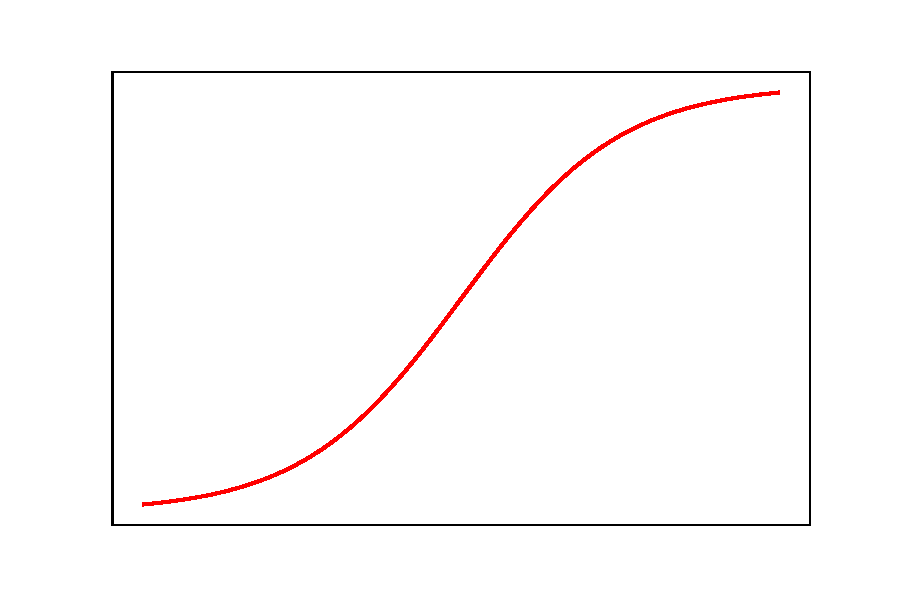
\includegraphics[width=0.15\textwidth]{img/sigmoid}}
				&
				$
					\begin{aligned}
						\sigma(z) = \frac{1}{1+e^{-x}}
					\end{aligned}
				$
				& $ (0,1) $\\
			\hline
			Unidade Linear Retificada	&
				\Centerstack{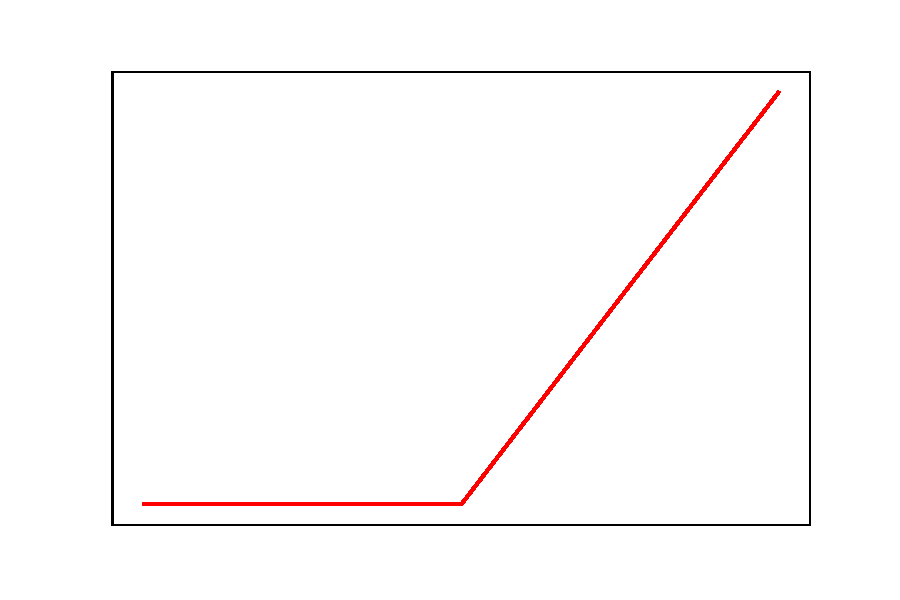
\includegraphics[width=0.15\textwidth]{img/relu}}
				&
				$
					\begin{aligned}
						\sigma(z) = max(0,z)
					\end{aligned}
				$
				& $ [0, \infty) $\\
			\hline
			Softmax					&
				\Centerstack{\includegraphics[width=0.15\textwidth]{img/softmax}}
				&
				$
					\begin{aligned}
						g(z_j) = \frac{e^{z_j}}{\sum^K_{j=1} e^{z_k}} \hspace{0.2cm}j=1, \ldots, K
					\end{aligned}
				$
				& $(-\infty, \infty)$\\
			\bottomrule
		\end{tabular}
	\end{adjustbox}
	\caption{Exemplos de funções de ativação}
\end{table}
. Todas estas alterações feitas ao modelo Perceptron inicial acabou por aumentar o escopo dos problema que podem ser resolvidos com RNAs.

\todo[inline]{aplicações}

As RNAs \emph{feedforward} formam a base para muitas aplicações, o que faz com que este modelo seja de extrema importância para profissionais da área de ML. Para exemplificar, as RNA convolucionais utilizadas para reconhecimento de objetos a partir de imagens são um tipo de RNAs \emph{feedforward}. Estas redes também são um pilar para as redes recorrentes, que alimentam muitas aplicações de linguagens naturais \cite{goodfellow2016deep}. Estes modelos filhos das RNAs \emph{feedforward} são parte da sub-área \emph{Deep Learning}, que será tratada na Seção \ref{sec:dl}.


\subsection{\emph{Deep Learning}}\label{sec:dl}
%!TEX root = ../../sbc-template.tex

\emph{Deep Learning} (DL), também conhecido como Aprendizagem Profunda, compreende um conjunto de técnicas de ML que podem ser aplicadas em problemas de aprendizado supervisionado e não-supervisionado. A principal característica dos modelos neste domínio é a capacidade de representar e reconhecer características sucessivamente complexas, por meio da adição de níveis ou camadas de operações não-lineares em sua arquiteturas, a exemplo das nas redes neurais profundas, máquinas de Boltzmann profundas e fórmulas proposicionais. Modelos deste tipo ganharam popularidade ao se mostraram capazes de resolver problemas complexos com um desempenho cada vez maior \cite{bengio2009learning}.

A melhoria do desempenho de modelos de DL é decorrente do aumento recente da quantidade de dados disponíveis sobre temas complexos, aliado ao aumento da disponibilidade de recursos computacionais para executar modelos mais robustos \cite{goodfellow2016deep,deng2014deep}. Alguns dados fornecidos pela IBM reforçam esta afirmação: em $2017$ foram gerados $2,5$ quintilhões de bytes de dados por dia, e $90\%$ do volume total de dados gerados até $2017$ no mundo foi criado somente nos últimos dois anos \cite{ibm2017bigdata}. Estes fatores possibilitaram a implementação de modelos que apresentaram uma melhoria exponencial na eficiência estatística frente a modelos mais rasos, devido a sua capacidade de organizar a computação através da composição de várias operações não-lineares, neste caso as funções de ativação, e uma hierarquia de características re-utilizadas, representadas pela adição de camadas \cite{goodfellow2016deep}.

Para exemplificar o efeito da adição de camadas aos modelos de DL, a Figura \ref{fig:compara_redes} mostra uma visão geral do aumento da profundidade das camadas de CNNs e o desempenho destas em problemas de detecção de objetos em imagens. Nota-se que, à medida que a profundidade aumenta, há uma diminuição no erro. Mais recentemente, isto também tem implicado na redução do número de parâmetros treináveis, através da implementação de técnicas de subamostragem \cite{haykin2009neural}. Este panorama reforça a hipótese de que o aumento da profundidade das CNNs impacta positivamente na captura de características e que estes avanços têm tornado as tarefas mais factíveis, com uma diminuição do esforço computacional associado, em comparação com modelos mais rasos \cite{goodfellow2016deep}.

\begin{figure}[ht]
	\centering
	\caption{Evolução de profunidade, taxa de erro e número de parâmetros das redes neurais profundas com o passar dos anos. Fonte: \cite{mediumcnn}.}
	\label{fig:compara_redes}
	\includegraphics[width=0.8\textwidth]{img/compara_redes.png}
\end{figure}

\subsubsection{Breve Histórico}

O termo \emph{Deep Learning} não é recente, foi utilizado pela primeira vez por Dechter, no contexto da descoberta de todas as configurações de conflitos mínimas a fim de resolver um problema de satisfação de restrições
\cite{dechter1986learning}. Porém, ganhou força a partir de pesquisas sobre RNAs \emph{feedforward} com muitas camadas ocultas, também conhecidas por redes neurais profundas \cite{deng2014deep}.

Considera-se que o desenvolvimento de DL pode ser entendido em três partes. Na primeira, houve a proposição de modelos lineares simples, compostos apenas por um neurônio, a exemplo dos neurônios de McCulloch e Pitts \cite{mcculloch1943logical} e \emph{Perceptron} de Rosenblatt  \cite{rosenblatt1958perceptron}. A segunda parte, iniciada nos anos 1980, teve como eixo central a interconexão entre vários neurônios e a proposição do algoritmo \emph{back-propagation} para ajuste de pesos no treinamento das RNAs  \cite{rumelhart1986parallel,rumelhart1986backpropagation}. Com estas contribuições, houve muita aplicação das RNAs em diversos domínios. Ainda no final deste segundo momento, duas contribuições relevantes foram feitas: os modelos \emph{Long Short-Term Memory} (LSTM) e LeNet, que utiliza o algoritmo de \emph{backpropagation} para treinar uma rede neural convolucional profunda para reconhecer dígitos escritos à mão
\cite{lenet}.

A terceira fase têm um marco inicial mais definido: compreende o ano de $2006$, quando Hinton utilizou o termo \emph{deep belief network} para designar um tipo de modelo de RNA MLP cujo treinamento adota uma estratégia gulosa e orientada a camadas, em inglês \emph{greedy layer-wise pretraining}. Cada camada é pré-treinada individualmente como maquina de Boltzmann restrita, e o modelo inteiro é então afinado utilizando técnicas de treinamento supervisionado, incluindo o algoritmo de \enph{backpropagation}. A partir daí, outros grupos de pesquisa passaram a investigar a técnica de Hinton, e com o tempo, o termo passou a designar modelos compostos de várias camadas sucessivas de operações não lineares utilizados para o aprendizado de determinada tarefa \cite{hinton2006fast, hinton2007learning, goodfellow2016deep, deng2014deep}.

Na conjectura atual, modelos de DL têm superado significativamente o estado da arte de modelos inteligentes em diversas competições em todo o mundo. A \emph{ImageNet Large Scale Visual Recognition Challenge} (ILSVRC) \cite{Imagenet} é uma competição em que equipes de pesquisa avaliam seus algoritmos em um conjunto de dados fornecido, e competem para chegar à melhor acurácia em várias tarefas de reconhecimento visual automático. O conjunto de dados, o ImageNet \cite{Imagenet}, consiste de um conjunto de aproximadamente $14$ milhões de imagens de $21$ mil itens organizados hierarquicamente, em que cada item contém no mínimo algumas centenas de imagens de exemplo. A performance dos modelos submetidos para a competição é chamada taxa de erro top-5, e representa o erro computado quando a classe alvo não se encontra entre as 5 apontadas pelo modelo como as que têm maior probabilidade de estarem na imagem. Em 2011, os melhores resultados de  classificação no ILSVRC tinham por volta de $25\%$ de erro top-5 nas tarefas propostas. Em 2012, o modelo AlexNet, uma rede neural convolucional proposta segundo as ideias de DL, atingiu apenas $16,4\%$ de erro, propondo um ganho dificilmente visto entre duas edições sucessivas da competição \cite{ImagenetChall:2012}.

O gráfico da Figura \ref{fig:compara_redes} sintetiza o histórico da competição ILSVRC, em que a partir do ano de 2012 houve a introdução de modelos baseados em DL, as redes neurais convolucionais, em inglês \emph{Convolutional Neural Networks} (CNNs). O histograma mostra a diminuição do erro na tarefa de aprendizado proposta e a linha laranja enfatiza o número de camadas ocultas utilizadas nos modelos vencedores.

\begin{figure}[ht]
	\centering
	\caption{Evolução do erro dos modelos vencedores da competição ILSVRC pela profundidade das redes neurais \cite{dl_ILSVRC, ImagenetChall}}
	\label{fig:compara_redes_ilsvrc}
	\includegraphics[width=0.8\textwidth]{img/compara_redes_ilsvrc.png}
\end{figure}

Apesar do foco inicial de DL ter sido concentrado no desenvolvimento de técnicas de aprendizado não-supervisionado e na habilidade de modelos profundos de boa generalização a partir de conjuntos de dados pequenos, o cenário atual das pesquisas nesta área consideram o uso de técnicas de aprendizado supervisionado, visando o endereçamento de conjuntos de dados massivos e categorizados, e também redes neurais profundas híbridas, que misturem técnicas e conceitos de ambas origens \cite{deng2014deep,goodfellow2016deep}. Nesta perspectiva encontram-se as CNNS, que apesar de terem impulsionado avanços na Visão Computacional desde a publicação da LeNet \cite{lenet}, têm capturado interesse intenso em aplicações de reconhecimento de objetos desde a divulgação dos resultados da ILSVRC 2012, cuja CNN ganhadora AlexNet \cite{alexnet} está na Figura \ref{fig:compara_redes_ilsvrc} \cite{deng2014deep}. Considerando esta importância, a seção a seguir compreenderá a explanação destes modelos, com especial para arquiteturas canônicas de maior destaque nos últimos anos.

\subsubsection{Redes Neurais Convolucionais} \label{subsubsec:rnc}

\emph{Redes Neurais Convolucionais} (CNN, do inglês \emph{Convolutional Neural Networks}) são uma classe de redes neurais \emph{feedforward} com topologia bem definida e estruturada em uma grade, com o uso de operações de convolução em pelo menos uma de suas camadas \cite{goodfellow2016deep}. Aplicadas em tarefas de classificação, regressão, localização, detecção e outras, este tipo de modelo se destaca no reconhecimento de padrões em dados de alta dimensionalidade, a exemplo de séries temporais, imagens e vídeos \cite{Khan:Livro}.

A operação de convolução possui um papel central nas CNNs. Esta operação descreve a média ponderada de uma determinada função $x_1(t)$ sob um intervalo fixo de uma variável, enquanto os pesos da média ponderada considerada pertencem à função $x_2(t)$ amostrados em intervalos $a$ \cite{bracewell1986fourier}. Assim, a convolução $s(t)$ de duas funções $x_1(t)$ e $x_2(t)$ é uma função $s: \mathds{Z} \rightarrow \mathds{R}$, denotada $s(t) = x_1(t) * x_2(t)$, e definida conforme Equação \ref{eq:int_convolucao} \cite{lathi2006sinais}:

\begin{equation}\label{eq:int_convolucao}
s(t) = x_1(t) * x_2(t) = \int_{-\infty}^{\infty} x_1(a) x_2(t-a)da.
\end{equation}

No contexto de ML, a função $x_1(t)$ é chamada de \emph{input}, a função $x_2(t)$ é o \emph{kernel}, e a saída $s(t)$ consiste no \emph{feature map}, ou mapa de características. No contexto prático, o \emph{input} normalmente é um vetor multidimensional de dados e o \emph{kernel} é um vetor multidimensional de pesos que devem ser ajustados para aprendizado das CNN. Considerando, por exemplo, uma imagem $I$ de dimensões $(m,n)$ como \emph{input} e a aplicação de um \emph{kernel} $K$, a versão discreta da convolução, passível de implementação computacional e equivalente à Equação \ref{eq:int_convolucao}, é mostrada na Equação \ref{eq:conv_img}:

\begin{equation}
 S(i,j) = I(i,j)*K(i,j) = \sum_{m}\sum_{n}I(m,n)K(i-m,j-n),\label{eq:conv_img}
\end{equation}
em que $S$ é o \emph{feature map} resultante e $(i,j)$ é a posição correspondente nesse mapa. Para otimizar os aspectos de implementação, os valores resultantes da operação de convolução são armazenados apenas nas posições $(i,j)$ explicitamente declaradas \cite{goodfellow2016deep}.

Os \emph{feature maps}, resultantes das operações de convolução, compreendem a noção de filtros, responsáveis por capturarem características relativas à entrada, tais como contornos, linhas, texturas, etc. Quando combinados de maneira sequencial, como proposto pelas CNNs, as características capturadas pelas camadas convolucionais vão se tornando mais complexas à medida que se aumenta a profundidade da rede. Assim, um primeiro \emph{feature map} de uma camada convolucional captura um simples contorno, enquanto um \emph{feature map} em uma camada mais profunda da rede pode capturar uma forma, um rosto ou até um objeto inteiro \cite{Buduma:Livro}. Esta noção é ilustrada na Figura \ref{fig:convolutions}.

\begin{figure}[!h]
	\centering
	\caption{Papel das camadas convolucionais e \emph{feature maps} nas CNNs. Fonte: \cite{Khan:Livro}.}
	\label{fig:convolutions}
	\includegraphics[width=0.8\textwidth]{./img/fundamenta/convolutions}
\end{figure}

As camadas convolucionais, que contém os \emph{feature maps} e os pesos da rede, normalmente são seguidas por funções de ativação como as exemplificadas na Seção \ref{sec:rnas}, mais especificamente na Tabela \ref{tab:ativacoes}. Via de regra, a toda camada convolucional em uma CNN, segue-se uma função de ativação, finalizando em uma operação de \emph{pooling}, como mostra a Figura \ref{fig:cnn_camada}.

\begin{figure}
	\centering
	\caption{Componentes de uma camada de uma rede neural convolucional \cite{goodfellow2016deep}.}
	\label{fig:cnn_camada}
	\includegraphics[height=0.3\textheight]{img/cnn_camada.png}
\end{figure}

 Uma função de \emph{pooling} substitui a saída da rede em determinada localização por uma síntese estatística das saídas vizinhas. Por exemplo, a operação \emph{max pooling} retorna o valor máximo em uma área retangular, enquanto a \emph{average pooling} retorna a média das saídas de um retângulo. O objetivo desta operação é fazer com que a representação ou \emph{feature map} seja invariante a pequenas translações (mudanças) na entrada. Invariante a translações significa que se a entrada for transladada por uma pequena quantia, os valores da maioria das saídas das funções de pooling vão continuar os mesmos. Esta invariância à translação local pode ser uma propriedade útil se a pessoa ligar mais pra ver se alguma característica está na imagem que dizer exatamente onde ela tá. Esta operação pode aumentar muito a eficiência estatística e reduções de requisitos de memória para guardar os parâmetros da rede, pois diminui a quantidade de parâmetros que serão passados para a próxima camada \cite{goodfellow2016deep}.

 Outros parâmetros, como \emph{padding} e \emph{strides}, são importantes para a captura de características. \emph{padding} consiste de adicionar um número de linhas e colunas em cada lado da entrada de maneira a controlar o tamanho do mapa de características resultante da operação de convolução. Já a distância entre duas janelas da convolução, ou da operação de \emph{pooling}, é medida através do número de \emph{strides}. Ambos parâmetros manipulam as dimensões das saídas das camadas de uma CNN \cite{chollet2017deep}.

\todo{Gancho?}
A seguir, serão apresentadas alguns modelos de CNNs que trouxeram grandes inovações para a área.

\subsubsection{Modelos Canônicos de Redes Neurais Convolucionais para Detecção de Objetos em Imagens} \label{subsubsec:modelos_canonicos}

Os modelos canônicos são arquiteturas que trouxeram contribuições importantes, pioneiras na aplicação de técnicas que são comuns ainda hoje no cenário de DL, e que são comumente utilizadas em diversas tarefas de aprendizado ainda hoje \cite{9dlpapers}.

A LeNet é o primeiro modelo de rede neural a aplicar convoluções ao invés das camadas totalmente conectadas convencionais. Foi proposta por LeCun em 1998, é composta de 7 camadas,incluindo a de entrada, duas convolucionais, duas de pooling, uma totalmente conectada e a saída. A tarefa de aprendizado endereçada por esta arquitetura foi o reconhecimento de dígitos. Para o treinamento e teste foi utilizado o conjunto de dados \emph{Modified National Institute of Standards and Technology} (MNIST), composto de 60000 imagens de treinamento e 10000 de teste dos dígitos de 0 a 9 escritos à mão. A LeNet foi amplamente utilizada por bancos para o reconhecimento de números escritos à mão em cheques digitalizado em imagens em escala de cinza de tamanho 32x32 \cite{lenet}. Apesar de pesquisas nesta área continuarem no decorrer dos anos, a quantidade insuficiente de bases de imagens catalogadas e o baixo poder computacional da época fizeram com que as CNNs permanecessem sem grandes destaques até 2012 \cite{dl9papers}.

AlexNet foi a primeira CNN ganhadora do desafio ILSVRC, em 2012, ao atingir um erro top-5 igual a $15.4\%$. O segundo melhor modelo daquele ano atingiu um erro de $26.2\%$. Esta rede, treinada para uma tarefa de classificação utilizando imagens de 1000 categorias da ImageNet, é formada por 5 camadas convolucionais com filtros de tamanho 11x11, intercaladas com camadas de \emph{max-pooling} e \emph{dropout} e 3 camadas totalmente conectadas. Utilizava a função de ativação \emph{ReLU} ao invés da tradicional tangente hiperbólica, técnicas de aumento de dados incluindo translações, reflexões horizontais e cortes nas imagens. Foi treinada utilizando duas GPU GTX 580 por 5 a 6 dias, com o algoritmo de \emph{backpropagation} utilizando gradiente descendente estocástico para \emph{batch} e técnicas como \emph{momentum} e \emph{weight decay}. Estas técnicas garantiram à rede um desempenho significativamente melhor que o dos modelos tradicionais que estavam sendo aplicados para a ILSVRC daquele ano \cite{alexnet}.

Uma CNN que ganhou destaque pela simplicidade e profundidade é a VGG. Apesar de não ter ganhado a ILSVRC 2014, alcançou um erro top-5 de $7.3\%$. Foi concebida na Universidade de Oxford, a VGG-19 contendo 19 camadas que utiliza estritamente filtros de 3x3 com \emph{stride} e \emph{pad} de 1, juntamente com \emph{max-pooling} de tamanho 2x2 e \emph{stride} 2. O número de filtros dobra após cada camada de \emph{max-pooling}, o que reforça a idéia de diminuir dimensões espaciais de largura e altura e aumentar a profundidade. A VGG-19 foi treinada em parte da ImageNet utilizando 4 GPUs Nvidia Titan Black por duas a três semanas \cite{vggnet}.

Uma das primeiras arquiteturas de CNNs que se desviou do caminho normal de simplesmente empilhar camadas convolucionais e de pooling em uma estrutura sequencial foi a GoogLeNet, também chamada de Inception. Dotada de 22 camadas convolucionais, a rede ganhou o ILSVRC 2014 com um erro top-5 de $6.7\%$. Esta performance se deve aos chamados de módulos Inception, compostos de camadas da rede que ocorremem paralelo. Ao invés de realizar uma operação de convolução ou \emph{max-pooling} de cada vez, várias operações diferentes são realizadas e os mapas de características obtidos são condensados e conectados ao próximo bloco Inception. A Figura \ref{fig:bloco_inception} mostra que há 4 conjuntos de operações a serem realizadas, todas contendo convoluções com filtros 1x1 em algum ponto, podendo haver também a convolução com filtros de tamanho 3x3, 5x5, ou uma operação de \emph{max-pooling} de 3x3. A convolução com filtro 1x1 é aplicada para reduzir a dimensionalidade do problema reduzindo a profundidade do mapa de características, além de retirar da entrada informações bem detalhadas em volume. As convoluções que utilizam filtros de 3x3 e 5x5 dão ao modelo a capacidade de extrair informações relevantes em larga escala. A camada de \emph{max-pooling} é aplicada a fim de reduzir a largura e altura do mapa de característas e combater \emph{overfitting}. Substitui as camadas totalmente conectadas por \emph{average pooling}, o que economiza um grande número de parâmetros. A rede, que foi treinada em algumas GPUs de alta performance em uma semana, utiliza ReLU como função de ativação e contem 9 módulos Inception com mais de 100 camadas no total. É capaz de realizar as funções das 4 operações diferentes enquanto ainda se mantém computacionalmente competitiva. Todas estas técnicas utilizadas para reduzir a dimensionalidade do problema surtiram efeito, pos a partir do gráfico mostrado na Figura \ref{fig:compara_redes} nota-se que esta rede tem 12 vezes menos parâmetros que a AlexNet \cite{inception}.

\begin{figure}
	\begin{subfigure}[h]{0.5\linewidth}
		\centering
		\caption{Bloco Inception. Fonte: \cite{9dlpapers}}
		\includegraphics[width=0.7\linewidth]{img/GoogLeNet}
		\label{fig:bloco_inception}
	\end{subfigure}
	\begin{subfigure}[h]{0.5\linewidth}
		\centering
		\caption{Bloco Residual. Fonte: COLOCAR FONTE}
		\includegraphics[width=0.7\linewidth]{img/resnets_modelvariants}
		\label{fig:bloco_residual}
	\end{subfigure} %
\end{figure}

A Microsoft ResNet foi a CNN vencedora do ILSVRC 2015, com uma taxa de erro top-5 de $3.6\%$. Composta de um total de 152 camadas, esta rede neural deve o sucesso de sua profundidade ao bloco residual, representado na Figura \ref{fig:bloco_residual}, que em sumo soma à saída de um bloco de convoluções uma saída de um bloco anterior, para que ambos \emph{feature maps} sejam alimentados à função de ativação ReLU. Em CNNs tradicionais, o mapa de características resultado de uma operação de convolução seguida de \emph{max-pooling} aplicada a uma entrada consista de uma representação nova que não mantém nenhuma informação da entrada original. O bloco residual faz com que esta entrada original persista em camadas mais profundas da rede. Isto garante que as características determinantes para a tarefa de aprendizado sejam disseminadas para camadas mais profundas, ao mesmo tempo em que mantém a dimensionalidade do problema reduzida se comparada com a GoogLeNet na Figura \ref{fig:compara_redes}, haja vista que nenhuma operação é feita em uma das vertentes do bloco residual. Outra razão para o bloco residual ser efetivo é que durante a fase \emph{backwards} o gradiente vai fluir mais facilmente pela rede, pois os blocos residuais estão diretamente conectados a camadas mais rasas na arquitetura, o que facilita a distribuição do gradiente. A ResNet foi treinada em 8 GPUs por duas a três semanas.

Observada a importânciaAs CNNs apresentadas nesta seção, vale notar que variantes destas redes pré-treinadas utilizando o conjunto ImageNet estão implementadas em bibliotecas como o \emph{Keras} \cite{keras:applications} e \emph{Tensorflow} \cite{tensorflow:models}, e são amplamente utilizadas para \emph{transfer learning}, com o objetivo de endereçar tarefas de aprendizado específicas. A técnica \emph{transfer learning} será elucidada a seguir.

\subsubsection{Transfer Learning}
As várias redes treinadas com milhares de classes de objetos da ImageNet e validadas no ILSVRC, a exemplo das citadas na Seção \ref{subsubsec:modelos_canonicos}, têm obtido alto desempenho nas tarefas de aprendizado endereçadas. É sabido que CNNs são modelos com um grande número de parâmetros que devem ser aprendidos a partir de exemplos de treinamento, cuja performance é limitada por conjuntos de dados relativamente pequenos. Neste contexto, nem sempre uma grande quantidade de imagens de exemplo estará disponível. Além disto, características distintas de um conjunto de dados, como iluminação, variações de ponto de vista e o fundo, inevitavelmente afetam o desempenho do reconhecimento ao treinar e testar em diferentes domínios. Assim, dada a natureza ávida por dados das CNNs e a dificuldade de consolidar conjuntos de dados em larga escala como o ImageNet, deve-se atentar para métodos que possibilitem a aplicação de CNNs em problemas com poucos dados.

Segundo Oquab em \cite{oquab2014learning}, representações de imagens aprendidas com CNNs a partir de conjuntos de dados com grande número de exemplos e categorias podem ser transferidas eficientemente para outras tarefas de reconhecimento visual que tenham uma quantidade limitada de dados de treinamento. Para isto, utiliza-se a técnica chamada \emph{transfer learning}, que consiste de transferir os conhecimentos entre domínios relacionados. No contexto das CNNs aplicadas em reconhecimento de objetos em imagens, as camadas internas podem agir como captores de características em médio nível. Estes podem ser pré-treinados na tarefa fonte, um conjunto de dados vasto como o ImageNet, e então re-utilizados na tarefa alvo, que pode conter um conjunto de dados mais restrito. No treinamento para a tarefa fonte a rede vai aprender a identificar linhas, contornos, objetos, e outras características, e então ser re-direcionada na tarefa alvo para aprender a identificar um grupo de objetos. Por exemplo, em \cite{zeiler2014visualizing}, treina-se a AlexNet de \cite{alexnet} no conjunto Imagenet, para então re-treiná-la em outros conjuntos de dados mais específicos.

Na prática, o \emph{transfer learinng} é feito ao transferir os parâmetros, $w$ e $b$, de um modelo já consolidado na literatura e pré-treinado com um conjunto de dados mais robusto, para um modelo similar ainda não treinado. Com o objetivo aproveitar os parâmetros pré-treinados, remove-se a última camada, ou seja, a camada de saída, e em seguida adiciona-se uma ou mais camadas novas, sem treinamento. Neste ponto, outros hiperparâmetros são adicionados ao modelo, como o número de camadas removidas do modelo original, número e tipos de camadas adicionadas ao novo modelo, quais camadas terão seus pesos inalterados ou congelados durante o re-treino, e ainda funções de ativação e outros fatores relativos às camadas adicionadas. Portanto, o modelo deve sofrer um ajuste fino em seus hiperparâmetro, ou \emph{fine tuning}, para que possa extrair as características do conjunto de dados da tarefa alvo de maneira satisfatória \cite{oquab2014learning}.

Tendo em vista a popularidade desta técnica, alguns exemplos da utilização de \emph{transfer learning} na tarefa de estimação de idade de pessoas a partir de imagens estão descritos na seção a seguir.


\subsection{Trabalhos Relacionados}\label{sec:trab_relac}
%!TEX root = ../sbc-template.tex

A aplicação de redes neurais convolutivas em problemas de classificação e detecção de objetos em imagens têm obtido resultados significativamente positivos. Em \cite{vggnet}, \cite{resnet}, \cite{inception}, \cite{redmon2016you}, \cite{ssd} e outros, são descritas arquiteturas robustas capazes de detectar dezenas de objetos em várias situações. Treinadas com conjuntos de dados visuais que contam com milhares de exemplos como a ImageNet, Pascal VOC e COCO, estas redes são conhecidas por seu bom desempelho. Algumas destas redes foram afinadas utilizando conjuntos de dados menores e especializados para a tarefa de estimação de idade aparente.

O trabalho de \cite{rothe2015dex} relata um método para estimação de idade aparente em imagens de faces imóveis utilizando \emph{deep learning}. Propõe-se um conjunto de $20$ redes neurais convolucionais classificadoras com arquiteturas VGG-16 pré-treinadas com a base de dados visuais ImageNet, e ajustadas utilizando imagens disponibilizadas pelo IMDB, Wikipedia, e o conjunto de dados \emph{Looking At People}--LAP para anotação de idade aparente. Cada modelo tem como saída um número discreto entre $0$ e $100$, representando a idade prevista. A saída final do modelo consiste na média entre as idades previstas pelos $20$ redes. A solução atingiu um MAE (\emph{Mean Average Error}) de $3.221$ na fase de testes.

Em \cite{liu2015agenet} cria-se um estimador composto pela fusão de um modelo regressor e outro classificador. A rede neural convolucional profunda \emph{GoogLeNet} (ou \emph{Inception}) \cite{inception} sofreu modificações em sua arquitetura, como adição de normalização do batch, remoção de camadas de \emph{dropout} e perda. O conjunto de modelos conseguiu prever idades com MAE de $3.3345$.

Ademais, é possível encontrar resultados satisfatórios para a tarefa de aprendizado proposta utilizando modelos menos complexos. Com o objetivo de consolidar um método de classificação de idade e gênero, \cite{levi2015age} propõe uma rede neural convolucional de natureza mais simples, se comparada com \cite{inception}, \cite{vggnet} ou \cite{resnet}. Sua arquitetura consiste em três camadas convolucionais com \emph{dropout} e funções de ativação \emph{ReLU}, seguidas por três camadas totalmente conectadas. A camada de saída tem como função de ativação a Softmax. A escolha por um design de rede menor é motivado pelo desejo de reduzir o risco de \emph{overfitting} e pela natureza do problema, que contém apenas 8 classes de idade. O modelo é treinado utilizando apenas o conjunto de referência \emph{Adience}, composto por imagens não filtradas para classificação de idade e gênero. Considerando uma margem de erro de uma classe vizinha, a melhor rede obteve acurácia de $84.7\% \pm 2.2$ ao empregar a técnica de sobre-amostragem.

